\chapter{Design and Implementation}
\label{chap:design}

This chapter walks through every component of \nidsname{} with
references to the actual source files. The order mirrors the
direction of data flow: a packet enters at the capture layer, is
processed by the dispatcher, is evaluated by the two detection
engines, may produce one or more alerts, and is finally persisted
and broadcast. The frontend, the API, the database schema and the
launcher are covered in their own sections after the core pipeline.

\section{General Architecture}
\label{sec:design-architecture}

\subsection{The Two-Tier Split}
\label{sec:design-tiers}

The system is split into a Python backend and a JavaScript
frontend. The split is the conventional one for modern web
applications: the backend owns the data, the business logic and the
detection engines; the frontend owns the rendering and the user
interaction. They communicate over HTTP for queries and over
WebSocket for live updates.

Both halves live in the same repository (\file{Licenta\_NIDS/}) but
are managed by separate package managers. The backend uses pip
through a virtual environment created at
\file{backend/.venv/}; the frontend uses npm through the standard
\file{frontend/node\_modules/} directory. The two installations are
orchestrated by the cross-platform launcher described in
Section~\ref{sec:design-launcher}.

\subsection{Packet Life Cycle}
\label{sec:design-lifecycle}

The path a packet takes from arrival to UI notification is short
enough to enumerate in eight steps:

\begin{enumerate}
  \item The packet enters either the Scapy \code{LiveSniffer} on a
    real network interface, or the in-process \code{TrafficSimulator}
    if simulation mode is enabled. Both paths converge on the same
    internal \code{Packet} dataclass.
  \item The packet handler --- a coroutine bound at startup ---
    invokes \code{Dispatcher.handle()} via
    \code{asyncio.run\_coroutine\_threadsafe} (in the case of the
    Scapy thread) or via a direct await (in the case of the
    simulator).
  \item \code{Dispatcher.handle()} updates the packet counter and
    the sliding-window packets-per-second meter, appends the packet
    to the in-memory ring buffer of size 200, and publishes a
    compact summary on the traffic event bus.
  \item Every fifth packet is sampled into a \code{TrafficEvent}
    row in the database. The sampling ratio is configurable
    (\code{TRAFFIC\_SAMPLE} constant in \file{dispatcher.py}); the
    default keeps the events table small enough for demo use.
  \item \code{Dispatcher.\_evaluate} runs the signature engine and,
    if a model is loaded, the ML detector. The two verdicts are
    merged into zero, one or several alert candidates, each carrying
    an explicit \code{detection\_method} field.
  \item Each candidate becomes an \code{Alert} row. The dispatcher
    writes the alert, generates a per-alert JSONL file with the
    last 50 packets from the ring buffer, writes a \code{PcapRecord}
    row indexing the file, and commits.
  \item The dispatcher publishes the alert payload on the alert
    event bus. Any WebSocket clients subscribed to
    \file{/ws/alerts} receive the payload immediately.
  \item The frontend's \code{useLiveAlerts} hook prepends the new
    alert to its in-memory list, which causes the dashboard live
    feed and the alerts page to re-render.
\end{enumerate}

Step (3) and step (4) run concurrently with step (5) only at the
asyncio level --- there is no thread-level parallelism inside the
dispatcher beyond the Scapy capture thread itself. The choice is
deliberate: a packet-level lock would have added complexity for no
measurable benefit at the throughput the validation workload
generates.

\begin{figure}[ht]
\centering
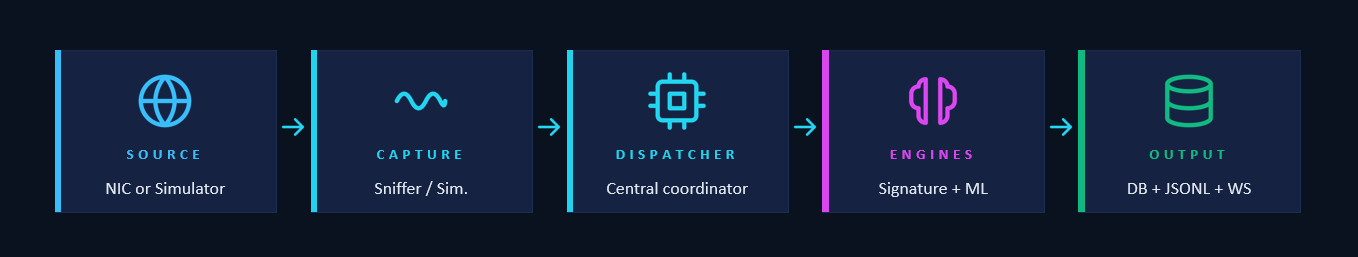
\includegraphics[width=\textwidth]{architecture-diagram}
\caption{High-level architecture: a packet enters at the source (a
NIC via Scapy, or the in-process simulator), is captured, handed to
the central dispatcher, evaluated by both the signature and ML
engines, and exits as a database row, a JSONL file on disk and a
WebSocket message to the browser.}
\label{fig:architecture}
\end{figure}

\section{Capture Layer}
\label{sec:design-capture}

The capture layer is the boundary between the outside world and the
detection pipeline. It is implemented as two interchangeable classes
in \file{backend/app/engine/sniffer.py}, both honouring the same
async callback contract:

\begin{lstlisting}[style=pyfile,caption={The capture-layer interface},label={lst:design-handler}]
PacketHandler = Callable[[Packet], Awaitable[None]]
\end{lstlisting}

\subsection{LiveSniffer (Scapy)}
\label{sec:design-livesniffer}

\code{LiveSniffer} wraps Scapy's blocking \code{sniff()} call on a
dedicated background thread. The thread is started with
\code{daemon=True} so it does not block process shutdown, and it
posts each parsed packet back to the FastAPI asyncio event loop via
\code{asyncio.run\_coroutine\_threadsafe(self.handler(pkt),
self.\_loop)}. The conversion from Scapy's nested layered structure
to the internal \code{Packet} dataclass happens in \code{\_to\_packet}:
the IP layer gives source and destination addresses, the TCP or UDP
layer gives ports, the TCP flags are extracted from the
\code{scapy\_pkt[TCP].flags} object and normalised to a
comma-separated string (\code{"S,A"} rather than the bitmask
\code{0x12}) so the signature engine can split them consistently
regardless of whether the source was Scapy or the simulator.

The class accepts a BPF filter via the constructor and forwards it
to \code{sniff(filter=...)}, which means uninteresting traffic is
dropped at the kernel boundary before reaching Python. Default is
empty (capture everything).

\subsection{TrafficSimulator}
\label{sec:design-simulator}

\code{TrafficSimulator} is the in-process packet generator. It runs
as an asyncio task started by the FastAPI lifespan handler and emits
two kinds of traffic: a benign baseline and on-demand attacks.

The benign baseline is controlled by the
\code{SIM\_BENIGN\_TRAFFIC} environment variable. When enabled, the
simulator emits 6--10 benign packets every 250\,ms (yielding a
steady 24--40 packets per second). Each benign packet has a random
source IP from the LAN client pool (\code{10.0.0.20} through
\code{10.0.0.59}), a destination of the configured defended host
(\code{DEFENDED\_HOST\_IP}, default \code{10.0.0.10}), a random
ephemeral source port, and one of the four common destination ports
(80, 443, 53, 22). The benign baseline is disabled by default so
the dashboard's live packet rate chart stays flat until the
operator deliberately enables traffic --- this makes the cause and
effect of attack injection visually obvious during demonstration.

The on-demand attacks are exposed through six factory methods, one
per attack family:

\begin{itemize}
  \item \code{\_nmap\_scan(attacker)} emits 25--40 TCP SYN packets
    sweeping 14 common service ports.
  \item \code{\_ssh\_brute(attacker)} emits 12--20 SYNs to port 22
    from a single source.
  \item \code{\_icmp\_flood(attacker)} emits 55--90 ICMP echo
    packets.
  \item \code{\_sqli(attacker)} emits one TCP packet containing the
    classic \texttt{' OR '1'='1} payload in an HTTP GET.
  \item \code{\_cmd\_inject(attacker)} emits one HTTP POST with
    shell metacharacters in the body.
  \item \code{\_reverse\_shell(attacker)} emits one TCP packet
    containing a \texttt{/bin/sh} redirection pattern.
\end{itemize}

All six are routed at the configured defended host. The choice of
attacker IP comes from a small pool
(\code{45.77.12.88}, \code{185.220.101.5}, \code{198.51.100.23});
the pool can be overridden by the API caller through the optional
\code{attacker} parameter on the \code{fire\_attack} method.

\subsection{Mode Selection}
\label{sec:design-mode}

The FastAPI lifespan handler in \file{backend/app/main.py} reads
the configuration and starts exactly one of the two capture sources.
The selection logic is:

\begin{lstlisting}[style=pyfile]
if settings.simulate_traffic or not settings.sniffer_interface:
    sim = TrafficSimulator(handler=dispatcher.handle, ...)
    sim.start()
    app.state.simulator = sim
else:
    try:
        live = LiveSniffer(...)
        live.start(asyncio.get_running_loop())
        app.state.sniffer = live
    except Exception as exc:
        log.warning("Live sniffer failed (%s). Falling back to simulator.", exc)
        sim = TrafficSimulator(handler=dispatcher.handle, ...)
        sim.start()
        app.state.simulator = sim
\end{lstlisting}

The fallback is important: if the operator forgets to install Npcap
on Windows, the application does not crash --- it logs a warning
and starts the simulator, so the dashboard always has data.

\section{The Dispatcher}
\label{sec:design-dispatcher}

The \code{Dispatcher} class in
\file{backend/app/engine/dispatcher.py} is the central coordination
point. It is instantiated once at startup by
\code{build\_dispatcher()} and stored as the module-level
\code{dispatcher} singleton plus on \code{app.state.dispatcher}.

The constructor takes the path to the PCAP output directory and a
flag indicating whether ML scoring is enabled. The instance holds
the packet counter, the alert counter, the ring buffer
(\code{deque(maxlen=200)}) and the sliding-window PPS tracker. The
core entry point is \code{handle()}, shown in
Listing~\ref{lst:design-handle}.

\begin{lstlisting}[style=pyfile,caption={Dispatcher entry point},label={lst:design-handle}]
async def handle(self, pkt: Packet) -> None:
    self._pkt_count += 1
    self._ring.append(pkt)
    self._tick_pps()

    await self._publish_traffic(pkt)
    await self._maybe_persist_event(pkt)

    alerts = self._evaluate(pkt)
    if alerts:
        await self._persist_and_broadcast(alerts)
\end{lstlisting}

The function reads like a flow diagram. Each helper method is
small (10--30 lines), pure with respect to its inputs, and easy to
unit-test. The same packet is observed by three independent
consumers (metrics, sampling, evaluation) without any of them
needing to know about the others.

\section{Signature Engine}
\label{sec:design-signature}

The signature engine lives in
\file{backend/app/engine/signatures.py}. It evaluates each packet
against the in-memory list of compiled rules and returns zero or
more alert candidates.

\subsection{Match Specification}
\label{sec:design-rule-spec}

A rule's \code{match} field is a JSON object with up to nine keys:

\begin{itemize}
  \item \code{protocol} --- \code{"tcp"}, \code{"udp"},
    \code{"icmp"} or \code{"any"}.
  \item \code{src\_ip} and \code{dst\_ip} --- single IP, CIDR
    notation, or \code{"any"}.
  \item \code{src\_port} and \code{dst\_port} --- single port,
    range string \code{"80-8080"}, list, or \code{"any"}.
  \item \code{flags} --- list of TCP flag letters that must all be
    set (e.g.\ \code{["S"]} for SYN-only, \code{["S","A"]} for
    SYN-ACK).
  \item \code{content} --- a case-insensitive substring search
    over the payload bytes.
  \item \code{regex} --- a Python regular expression evaluated
    against the payload decoded as UTF-8 with replacement.
  \item \code{min\_length} --- a minimum frame length in bytes.
  \item \code{threshold} --- a sub-object with \code{count},
    \code{seconds} and \code{track} fields turning the rule into a
    sliding-window counter.
\end{itemize}

The default rule set is seeded from
\file{backend/data/rules/default\_rules.yaml}. The ten bundled
rules cover the six attack families used in the validation
scenario plus a few demonstration rules (suspicious TLS SNI,
plaintext Telnet, oversized UDP). The full YAML for the Nmap rule
illustrates the format:

\begin{lstlisting}[style=yamlfile,caption={The Nmap scan rule, as stored in the seed YAML},label={lst:design-nmap-rule}]
- name: "Nmap TCP SYN scan"
  description: "High rate of TCP SYN packets from a single host (port scan signature)."
  category: "Reconnaissance"
  severity: "medium"
  action: "alert"
  match:
    protocol: "tcp"
    flags: ["S"]
    threshold:
      count: 8
      seconds: 5
      track: "src_ip"
\end{lstlisting}

\subsection{Threshold Tracking}
\label{sec:design-threshold}

The threshold logic is implemented by a small helper class,
\code{\_ThresholdTracker}, which maintains a sliding window of
event timestamps keyed by the tuple (\emph{rule id}, \emph{track
value}). When a rule with a threshold fires, the tracker appends
the current monotonic timestamp to the appropriate deque, drops any
entries older than the configured window, and returns
\code{True} if the deque length has reached the configured count.

The tracker uses \code{time.monotonic()} rather than wall-clock
time, so that NTP adjustments do not perturb the window. For the
Nmap rule with \code{count=8, seconds=5}, an attacker who sends 8
SYNs within any five-second period will trigger an alert; an
attacker who paces the scan with a 700-millisecond delay between
probes will not.

\subsection{Evaluate Loop}
\label{sec:design-evaluate-loop}

The \code{evaluate()} method iterates the compiled rules and
applies each predicate in order:

\begin{enumerate}
  \item Protocol match (or \code{any}).
  \item Source IP / CIDR match.
  \item Destination IP / CIDR match.
  \item Source port match (single, range, list).
  \item Destination port match.
  \item TCP flag subset match.
  \item Content substring (case-insensitive).
  \item Regex search.
  \item Minimum frame length.
  \item Threshold (if present) --- only the last step that actually
    increments any state.
\end{enumerate}

The order is deliberate: cheap checks first, expensive ones last.
A rule that does not match the protocol is dismissed in a single
string comparison; the regex check, which is the most expensive,
only runs for rules where all the cheaper predicates already
passed.

\section{Machine-Learning Detector}
\label{sec:design-ml}

The ML detector in \file{backend/app/engine/ml\_detector.py}
implements the two algorithms behind a common interface.

\subsection{Feature Vector}
\label{sec:design-features}

Each packet is converted into a six-dimensional NumPy array. The
features were chosen to be cheap to extract (no payload parsing,
no protocol-aware analysis) and to encode the kinds of behaviour
the attack catalogue actually exhibits:

\begin{enumerate}
  \item \code{src\_port} --- source port number.
  \item \code{dst\_port} --- destination port number.
  \item \code{length} --- L2 frame length in bytes.
  \item \code{proto\_id} --- 6 for TCP, 17 for UDP, 1 for ICMP, 0
    otherwise. Matches the IANA protocol numbers.
  \item \code{flag\_mask} --- a bitmask of the TCP flags (FIN=1,
    SYN=2, RST=4, PSH=8, ACK=16, URG=32). For non-TCP packets it
    is zero.
  \item \code{inter\_arrival\_ms} --- the gap in milliseconds since
    the previous packet from the same source IP. Maintained as
    streaming state in a dictionary inside the detector.
\end{enumerate}

The choice was conservative on purpose. A six-feature vector is
small enough to inspect by hand on the Alert Detail page, and it
avoids the dataset-leakage trap that more elaborate feature sets
fall into~\cite{sommer2010outside}.

\subsection{Training}
\label{sec:design-ml-train}

The \code{train\_synthetic()} method generates a 4000-sample
training set with a 70/30 split between normal and malicious
classes. The normal class uses random draws from distributions that
mimic the benign baseline (typical ports, moderate frame sizes,
exponential inter-arrival around 200\,ms). The malicious class uses
distributions skewed toward the attack patterns (high ephemeral
source ports, attack-favourite destination ports, very small or
very large frames, short inter-arrival times).

Both algorithms train on a 75/25 train-test split.
\code{RandomForestClassifier(n\_estimators=200, max\_depth=12,
random\_state=42)} fits in roughly one second on a mid-range
laptop. \code{IsolationForest(n\_estimators=200, contamination=0.3,
random\_state=42)} fits in roughly 0.7 seconds and only sees the
normal-class samples during training.

Both produce four classification metrics (accuracy, precision,
recall, F1) on the held-out test set. Random Forest also exposes
\code{feature\_importances\_}, which the API surfaces in the
\code{MLModelOut} response and the frontend renders as a Recharts
bar chart on the ML Models page.

\begin{figure}[ht]
\centering
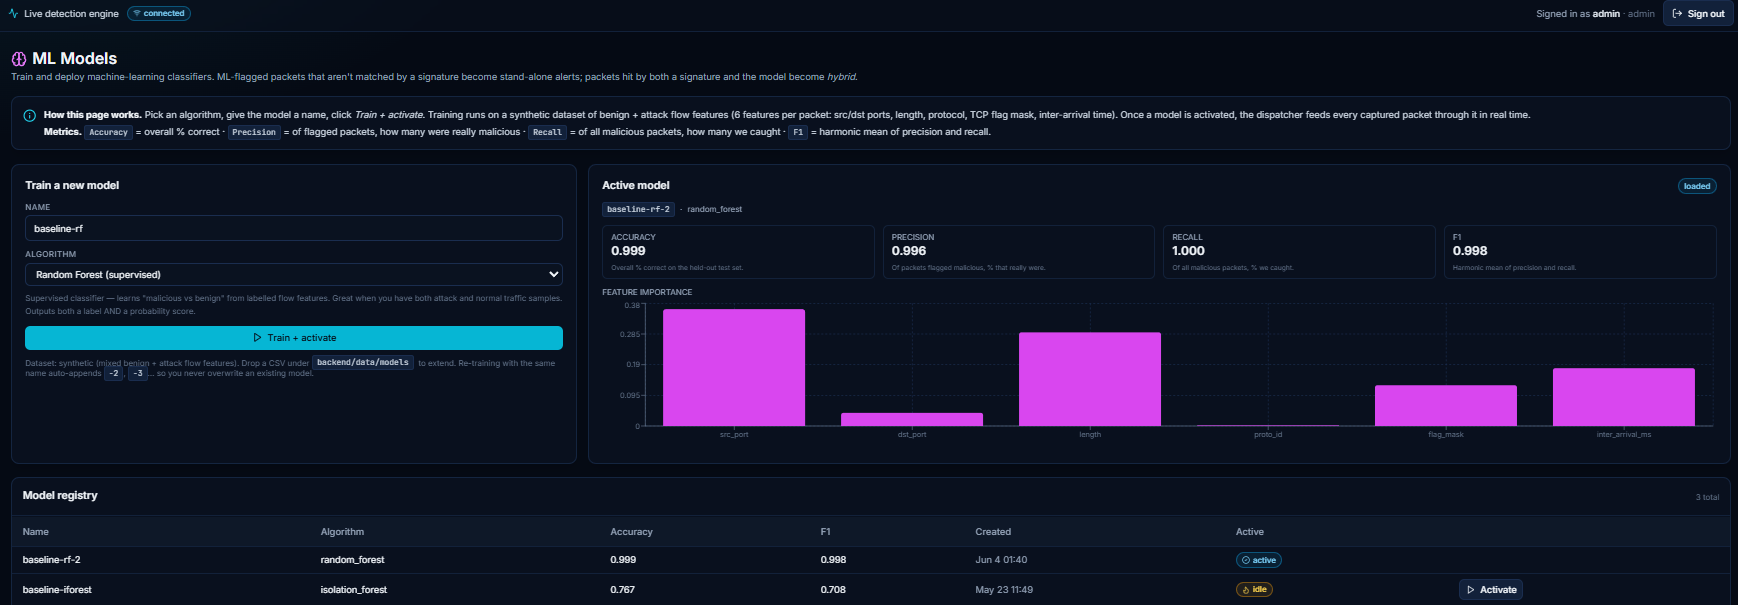
\includegraphics[width=\textwidth]{ml-models}
\caption{The ML Models page after training the default Random
Forest classifier. The four metric cards report accuracy,
precision, recall and F1 on the held-out test split; the bar chart
shows the per-feature importance derived from the model's
\code{feature\_importances\_} attribute, with \code{src\_port} and
\code{length} carrying the most discriminative signal.}
\label{fig:ml-models}
\end{figure}

\subsection{Inference}
\label{sec:design-ml-infer}

The \code{score(pkt)} method extracts the feature vector for the
incoming packet, runs it through the active model and returns a
\code{(label, score)} tuple. For Random Forest the score is
\code{predict\_proba()[0][1]}; for Isolation Forest it is the
negative of \code{decision\_function()[0]}, so larger values mean
more anomalous. The label is 1 (malicious) if the score is at or
above the threshold, 0 (benign) otherwise.

The inference path is wrapped in a mutex
(\code{threading.Lock}) so that training and scoring cannot race.
In practice training is not concurrent with high-volume scoring
since it is triggered by an explicit API call, but the lock makes
the code obviously safe.

\section{Hybrid Merge Logic}
\label{sec:design-detection}

The merge logic is the heart of the system. It lives in
\code{Dispatcher.\_evaluate} and is shown in
Listing~\ref{lst:design-merge}.

\begin{lstlisting}[style=pyfile,caption={Hybrid alert merge logic},label={lst:design-merge}]
def _evaluate(self, pkt: Packet) -> list[dict[str, Any]]:
    signature_hits: list[dict[str, Any]] = list(engine.evaluate(pkt))

    ml_label, ml_score = 0, 0.0
    if self.enable_ml and detector.is_active():
        ml_label, ml_score = detector.score(pkt)

    # ML-only alert: signature engine missed, ML score is high enough
    if ml_label == 1 and ml_score >= ML_ALERT_THRESHOLD and not signature_hits:
        return [self._ml_candidate(pkt, ml_score)]

    # Hybrid upgrade: both engines agreed
    if signature_hits and ml_label == 1:
        for h in signature_hits:
            h["detection_method"] = "hybrid"
            h["ml_score"] = ml_score
            h["ml_label"] = "malicious"

    return signature_hits
\end{lstlisting}

The function is twenty lines long and contains every alerting
decision the system makes. A signature-only alert is emitted when
the signature engine matched and the ML model either disagreed or
was not active. An ml-only alert is emitted when the signature
engine missed and the ML model scored above
\code{ML\_ALERT\_THRESHOLD} (0.8 by default). A hybrid alert is
the same row as the signature hit, with the detection method
upgraded and the ML score attached.

\section{Forensics Module}
\label{sec:design-forensics}

The forensics module is implemented by the small helper
\code{write\_packet\_log} in
\file{backend/app/engine/forensics.py}, plus a few lines in the
dispatcher's \code{\_persist\_and\_broadcast()} method that invoke
it.

When an alert is created, the dispatcher takes the last 50 entries
from the ring buffer
(\code{list(self.\_ring)[-SNAPSHOT\_TAIL:]}), passes them and the
alert ID to \code{write\_packet\_log()}, and stores the returned
file path on both the \code{Alert} row and the corresponding
\code{PcapRecord} row. The file is JSON Lines: one packet per
line, encoded as a JSON object with the timestamp, the 5-tuple,
the TCP flags, the frame length and the first 256 bytes of the
payload (decoded as UTF-8 with replacement, since binary protocols
do not decode cleanly).

The file name pattern is \code{alert\_\{alert\_id\}\_\{epoch\}.jsonl}.
A typical file might be 7\,kB for a 50-packet snapshot, which is
small enough that the application can keep thousands of them
without disk-space concerns.

\subsection{Downloading from the UI}
\label{sec:design-forensics-download}

The download endpoint at
\code{GET /api/forensics/alert/\{alert\_id\}/download} returns the
file with \code{FileResponse}. Because the endpoint is protected
by \code{Depends(get\_current\_user)}, the frontend cannot
simply emit a plain \code{<a href download>} link --- the anchor
navigation would not carry the JWT in the \code{Authorization}
header and the server would return 401.

The frontend handles this with the \code{apiDownload(url,
filename)} helper in \file{frontend/src/api/client.js}: it issues
a \code{fetch(url, \{headers: \{Authorization: 'Bearer ' + token\}\})},
wraps the response body in a \code{Blob}, calls
\code{URL.createObjectURL} and triggers a synthetic anchor click.
This pattern is the standard workaround for authenticated
downloads from a Single-Page Application and resolved the
``download.json --- File wasn't available on site'' error I
encountered during development.

\begin{figure}[ht]
\centering
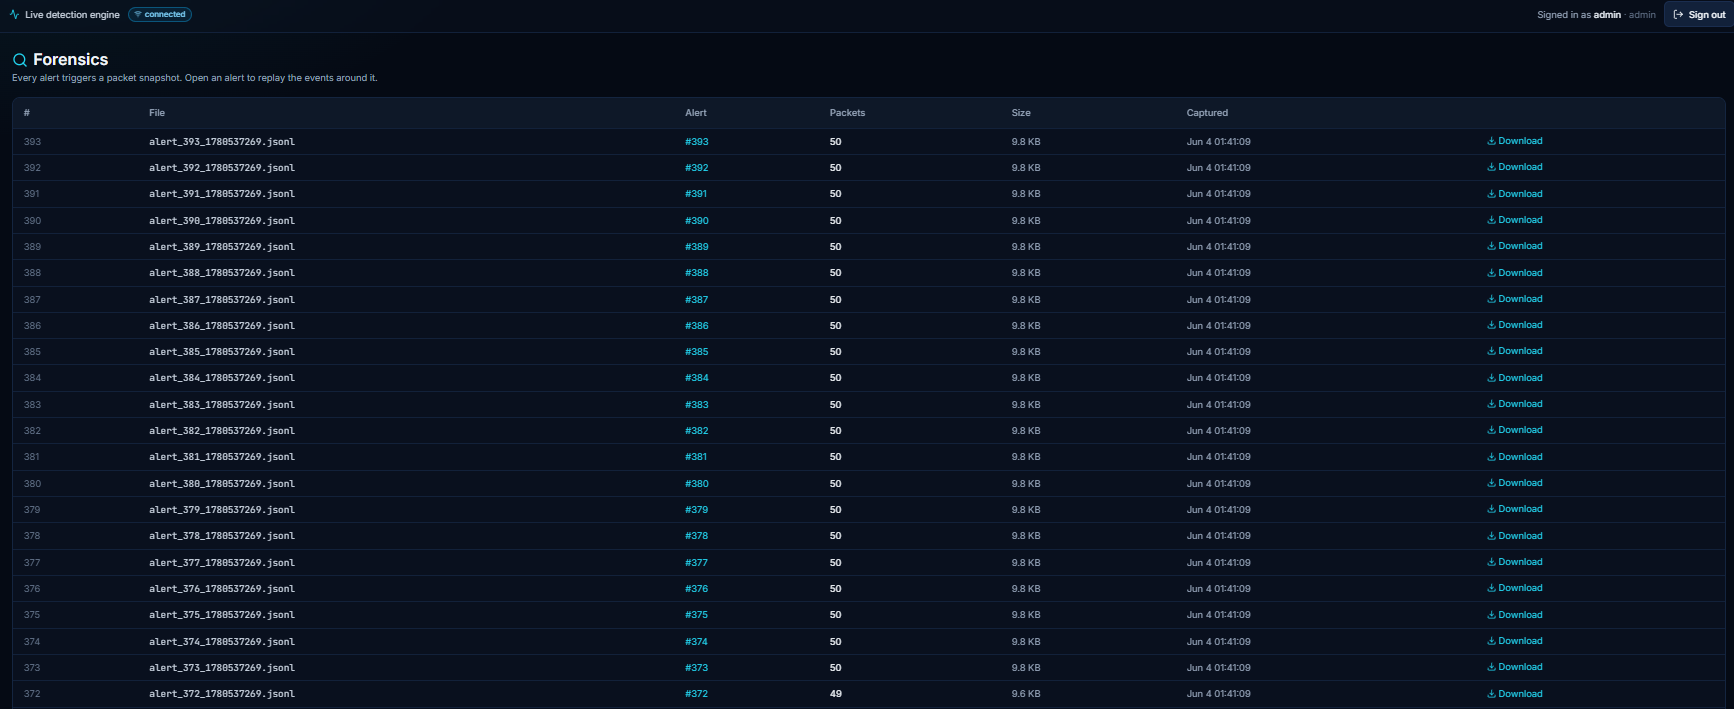
\includegraphics[width=\textwidth]{forensics}
\caption{The Forensics page listing the JSONL captures stored on
disk. Each row corresponds to one alert and carries a link to the
underlying \code{Alert} record plus a Download button that uses
the authenticated \code{apiDownload} helper. In this run the
dispatcher has accumulated several hundred captures, each holding
50 packets at roughly ten kilobytes per file.}
\label{fig:forensics}
\end{figure}

\section{REST and WebSocket API}
\label{sec:design-api}

The HTTP surface is organised by FastAPI routers, one per
resource type, all mounted in \file{backend/app/main.py}. The
routers are:

\begin{itemize}
  \item \file{api/auth.py} --- login, current-user, change
    password.
  \item \file{api/alerts.py} --- list (with filters), get,
    update status.
  \item \file{api/rules.py} --- list, create, update, delete.
  \item \file{api/dashboard.py} --- aggregated metrics for the
    dashboard summary.
  \item \file{api/forensics.py} --- list captures, get packets,
    download file.
  \item \file{api/ml.py} --- list models, train, activate, status.
  \item \file{api/sim.py} --- attack catalogue, fire attack,
    toggle benign traffic.
\end{itemize}

Every router (except \file{auth.py}) declares
\code{dependencies=[Depends(get\_current\_user)]} at the
router level, so every endpoint inherits the authentication
requirement without having to repeat it on every route. The
dependency is one of the cleanest things FastAPI does: it
decodes the JWT, loads the user from the database, and either
injects the \code{User} into the route parameters or raises an
HTTPException that becomes a clean 401 response.

The WebSocket endpoints live in
\file{backend/app/ws/alerts.py}. Authentication on these
endpoints is awkward because browsers cannot set custom request
headers on WebSocket opens; \nidsname{} solves this by accepting
the JWT as a query parameter (\code{ws://host/ws/alerts?token=...}).
The handler decodes the token before subscribing the connection
to the relevant event bus, exactly mirroring the REST behaviour.

The two buses (\code{alert\_bus} and \code{traffic\_bus}, defined
in \file{backend/app/engine/bus.py}) are simple asyncio
publish-subscribe primitives: each subscriber holds an
asyncio queue, and the bus's \code{publish()} method writes the
event to every subscriber's queue. The \code{/ws/traffic}
endpoint additionally batches and throttles traffic events
(up to 50 per batch, flushed every 500\,ms) so the chart in the
browser does not get bombarded with hundreds of single-packet
messages per second under heavy load.

\section{Frontend}
\label{sec:design-frontend}

The frontend is a React 18 single-page application bundled by
Vite. The source tree is small enough to enumerate:

\begin{itemize}
  \item \file{src/api/client.js} --- HTTP and WebSocket helpers,
    plus the authenticated \code{apiDownload} discussed above.
  \item \file{src/store/auth.jsx} --- the authentication
    \code{AuthContext} with login, logout and JWT persistence in
    \code{sessionStorage}.
  \item \file{src/hooks/useLiveAlerts.js} and
    \file{src/hooks/useLiveTraffic.js} --- the two WebSocket
    subscriber hooks, both used by the shared layout.
  \item \file{src/components/Layout.jsx} --- the sidebar plus
    main content frame; also where the live WebSocket
    subscriptions live so they survive page navigation.
  \item \file{src/components/Sidebar.jsx},
    \file{components/TopBar.jsx},
    \file{components/SeverityBadge.jsx},
    \file{components/MethodBadge.jsx},
    \file{components/StatCard.jsx},
    \file{components/ConfirmDialog.jsx} --- the shared widget set.
  \item \file{src/pages/*.jsx} --- one file per page (Login,
    Dashboard, Alerts, AlertDetail, Rules, MLModels, Forensics,
    AttackConsole, Settings).
\end{itemize}

\subsection{Authentication and Routing}
\label{sec:design-routing}

The router (\code{App.jsx}) wraps every non-login route in a
\code{RequireAuth} component that reads the auth context and
redirects to \file{/login} if no user is present. The
\code{AuthProvider} restores the token from
\code{sessionStorage} on mount, calls \code{GET /api/auth/me} to
hydrate the user, and unsets the token on a 401 response.

A subtle resilience improvement I added during development is a
small retry loop inside the \code{login} function: transient
5xx responses (which can happen on cold-boot races against the
backend's lifespan handler) are retried up to three times with
linear backoff before the failure is surfaced to the user. The
behaviour eliminates the ``Internal server error --- press the
button again'' artefact that briefly affected the first request
after a fresh deployment.

\subsection{Live Data Lifting}
\label{sec:design-live-context}

The two live hooks (\code{useLiveAlerts} and \code{useLiveTraffic})
are mounted at the \code{Layout} level rather than inside the
individual pages. The reason is state preservation: hooks mounted
inside a page are torn down when the user navigates away, and any
ring buffer they maintain is reset. By moving them up to the
shared layout, the live data persists across all routes, which
fixed the bug where the live packet-rate chart on the dashboard
reset to zero every time the user came back from the alerts
page.

The shared context exposes a single object with four properties:
\code{alerts}, \code{connected}, \code{traffic} and
\code{trafficConnected}. Each page that needs live data reads
exactly what it needs via the \code{useLive()} helper.

\subsection{Pages}
\label{sec:design-pages}

The eight pages of the console are described below, each
illustrated by a screenshot from a running instance.

\textbf{Login} (\file{Login.jsx}) is a single form bound to the
\code{login} action. Default credentials (\code{admin} / \code{admin})
are seeded by the backend on first boot. The deep-navy background
and the cyan shield emblem set the visual identity used across the
rest of the console; the small ``Default credentials'' hint at the
bottom of the form is removed when the application is deployed in
production via the \code{DEBUG=false} flag.

\begin{figure}[ht]
\centering
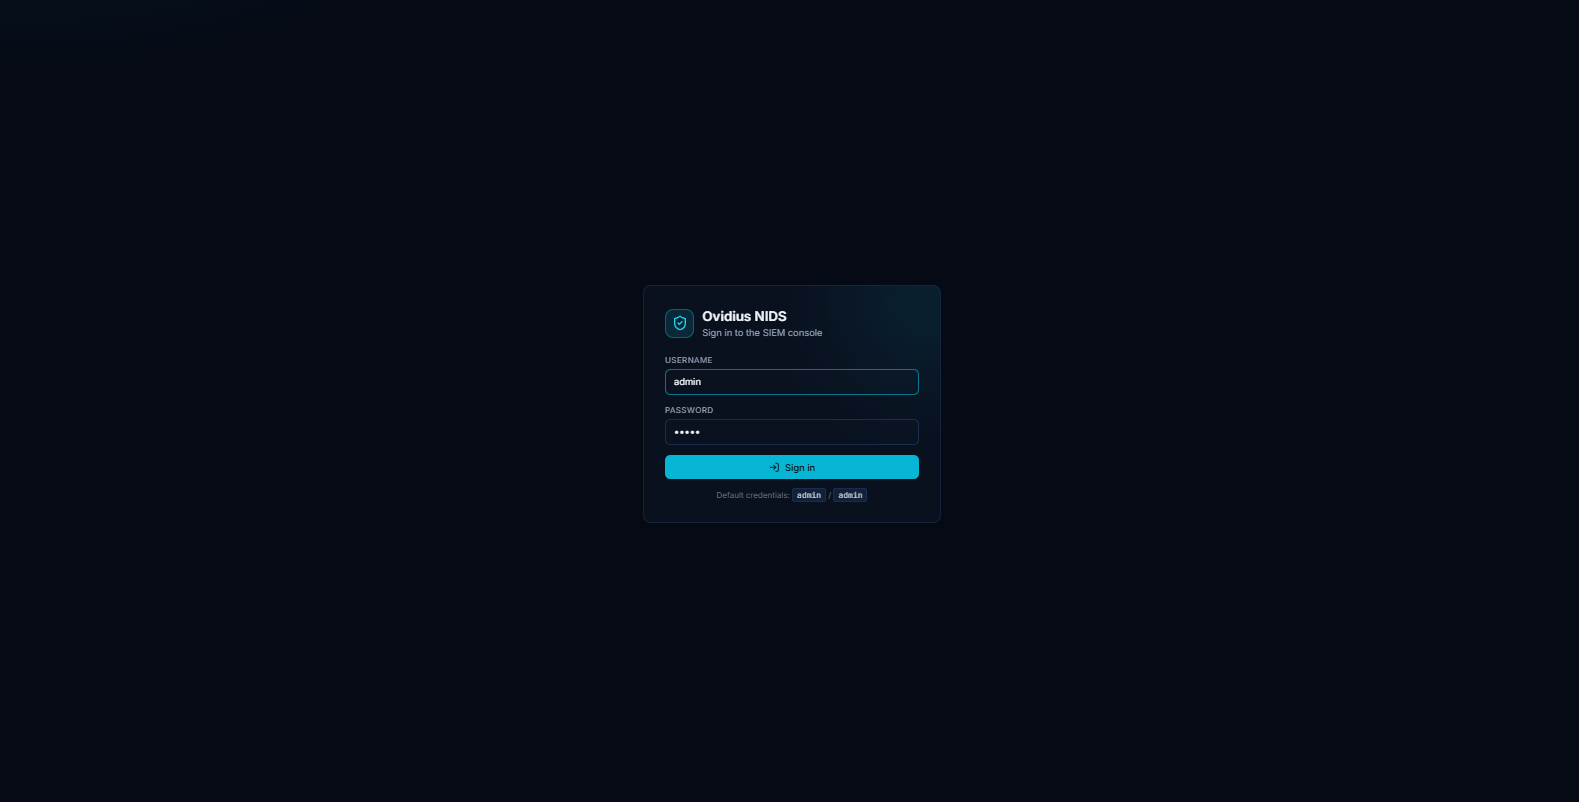
\includegraphics[width=0.6\textwidth]{login}
\caption{The Login page. A single form with the OAuth2 password
flow against \code{POST /api/auth/login}; on success the token is
written to \code{sessionStorage} and the user is redirected to
the Dashboard.}
\label{fig:login}
\end{figure}

\textbf{Dashboard} (\file{Dashboard.jsx}) is the operations
overview. The top row is four KPI cards (24-hour alert count,
open alerts, packet count, packets per second), pulled from
\code{/api/dashboard/summary} every five seconds. The middle row
is the live packet-rate area chart (from the WebSocket) and a
severity distribution pie. The bottom row is the 6-hour alert
timeline (10-minute buckets), a detection method pie, and three
small panels for top source IPs, top destination ports and the
live alert feed. The ``Monitoring host'' badge in the top right is
a single source of truth for which host the operator is watching
--- it pulls the \code{defended\_host\_ip} from
\code{/api/health} and the colour-codes the mode (simulator versus
live capture).

\begin{figure}[ht]
\centering
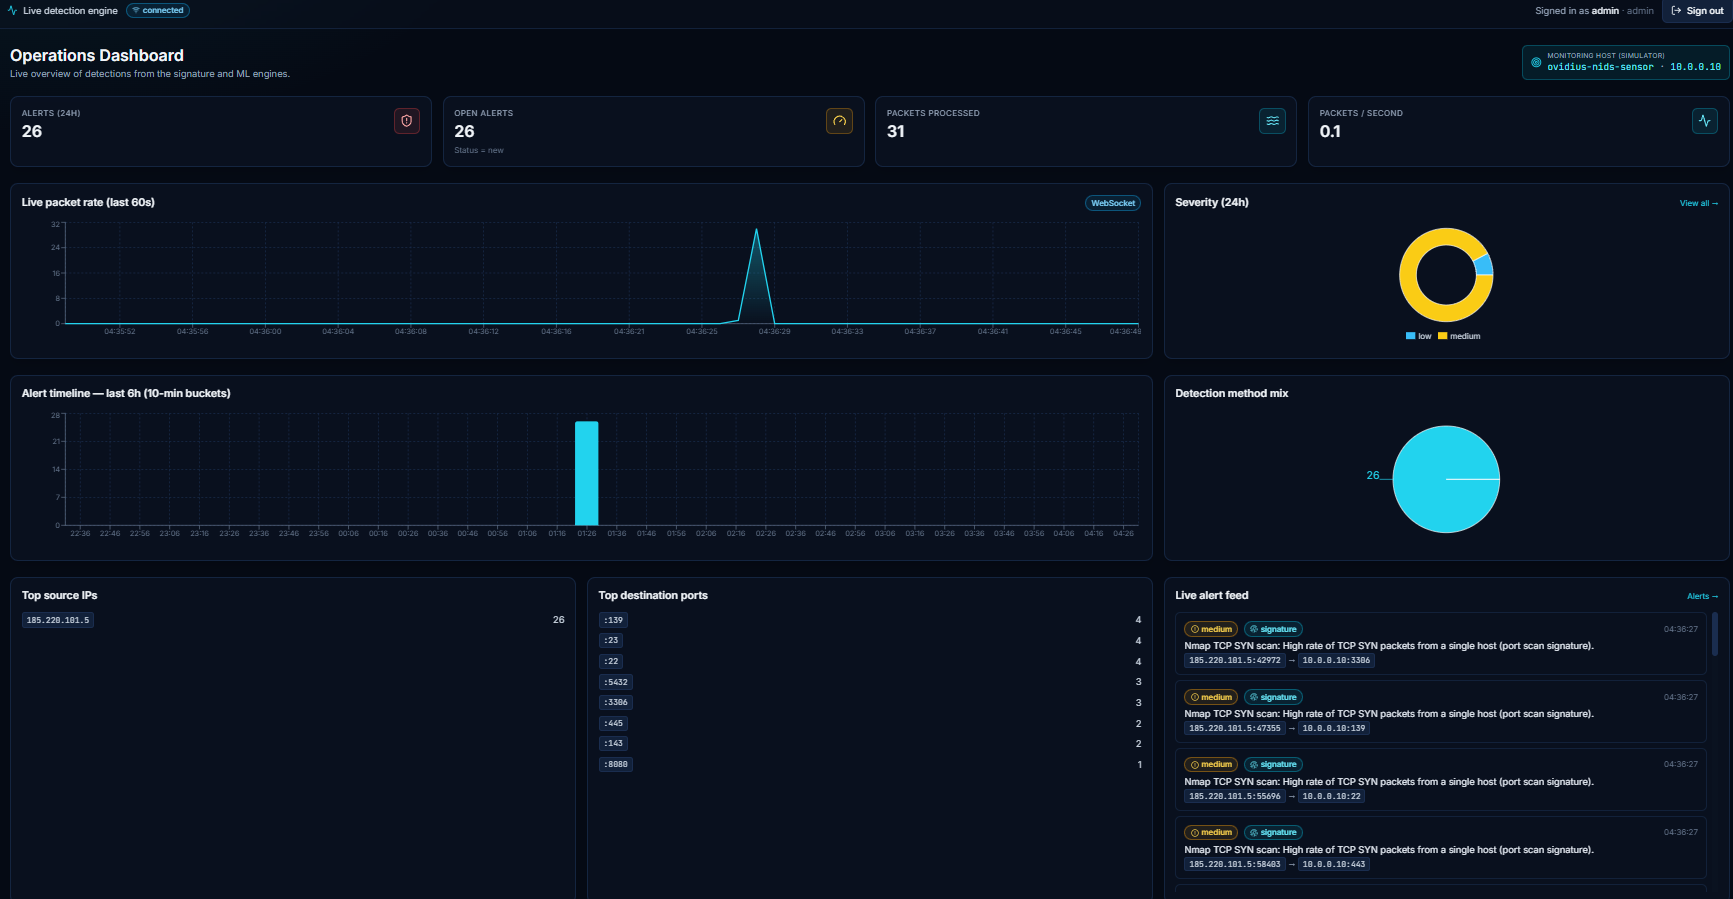
\includegraphics[width=\textwidth]{dashboard}
\caption{The Operations Dashboard. The visible spike on the live
packet-rate chart is a single attack burst injected through the
Attack Console; the 26 alerts produced by that burst show up
across the severity pie, the 6-hour timeline (the tall bar around
01:30), the detection-method pie and the live alert feed on the
right.}
\label{fig:dashboard}
\end{figure}

\textbf{Alerts} (\file{Alerts.jsx}) is the triage table. Filters
for severity, detection method, status and free-text search work
on both the historical rows fetched from \code{/api/alerts} and
on the live WebSocket stream prepended to the table. Each row
has a status dropdown (new / triaged / closed) and an Inspect
link to the detail page. The filter widgets are debounced ---
the search field re-fetches 300\,ms after the last keystroke
rather than on every character, which is the canonical
optimisation for an input-driven query.

\begin{figure}[ht]
\centering
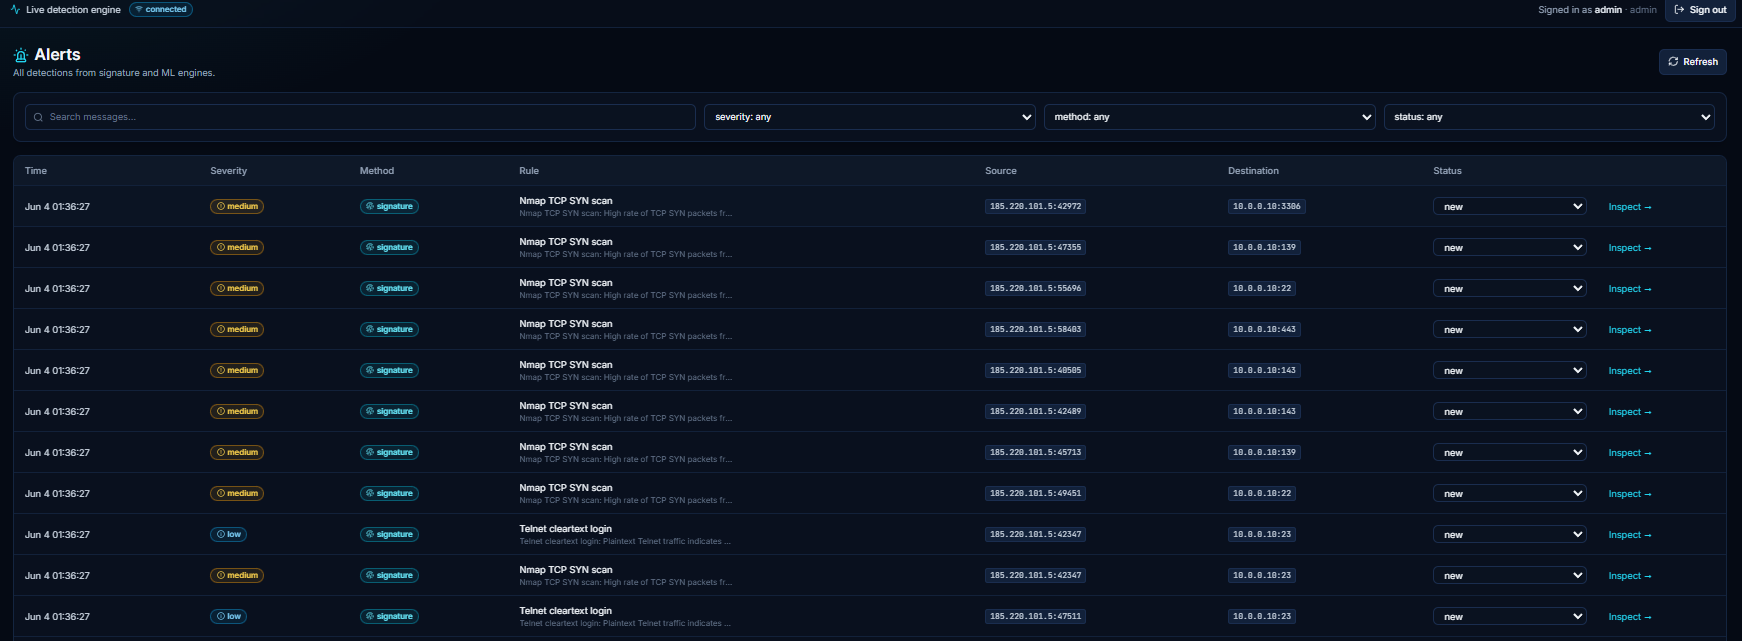
\includegraphics[width=\textwidth]{alerts}
\caption{The Alerts page after a port-scan burst. Every row's
detection method is \code{signature} and the source IP matches
the synthetic attacker pool (\code{185.220.101.5}); the
destination IP \code{10.0.0.10} is the configured defended host.
The two \code{Telnet cleartext login} entries are a different
rule that happened to fire on traffic to port 23 from the same
attacker burst.}
\label{fig:alerts}
\end{figure}

\textbf{Alert Detail} (\file{AlertDetail.jsx}) shows the full
record for one alert: severity, detection method, source and
destination, payload preview, the path of the JSONL capture, and
a table of the captured packets with their flags and lengths.
The Download button uses the authenticated \code{apiDownload}
helper.

\begin{figure}[ht]
\centering
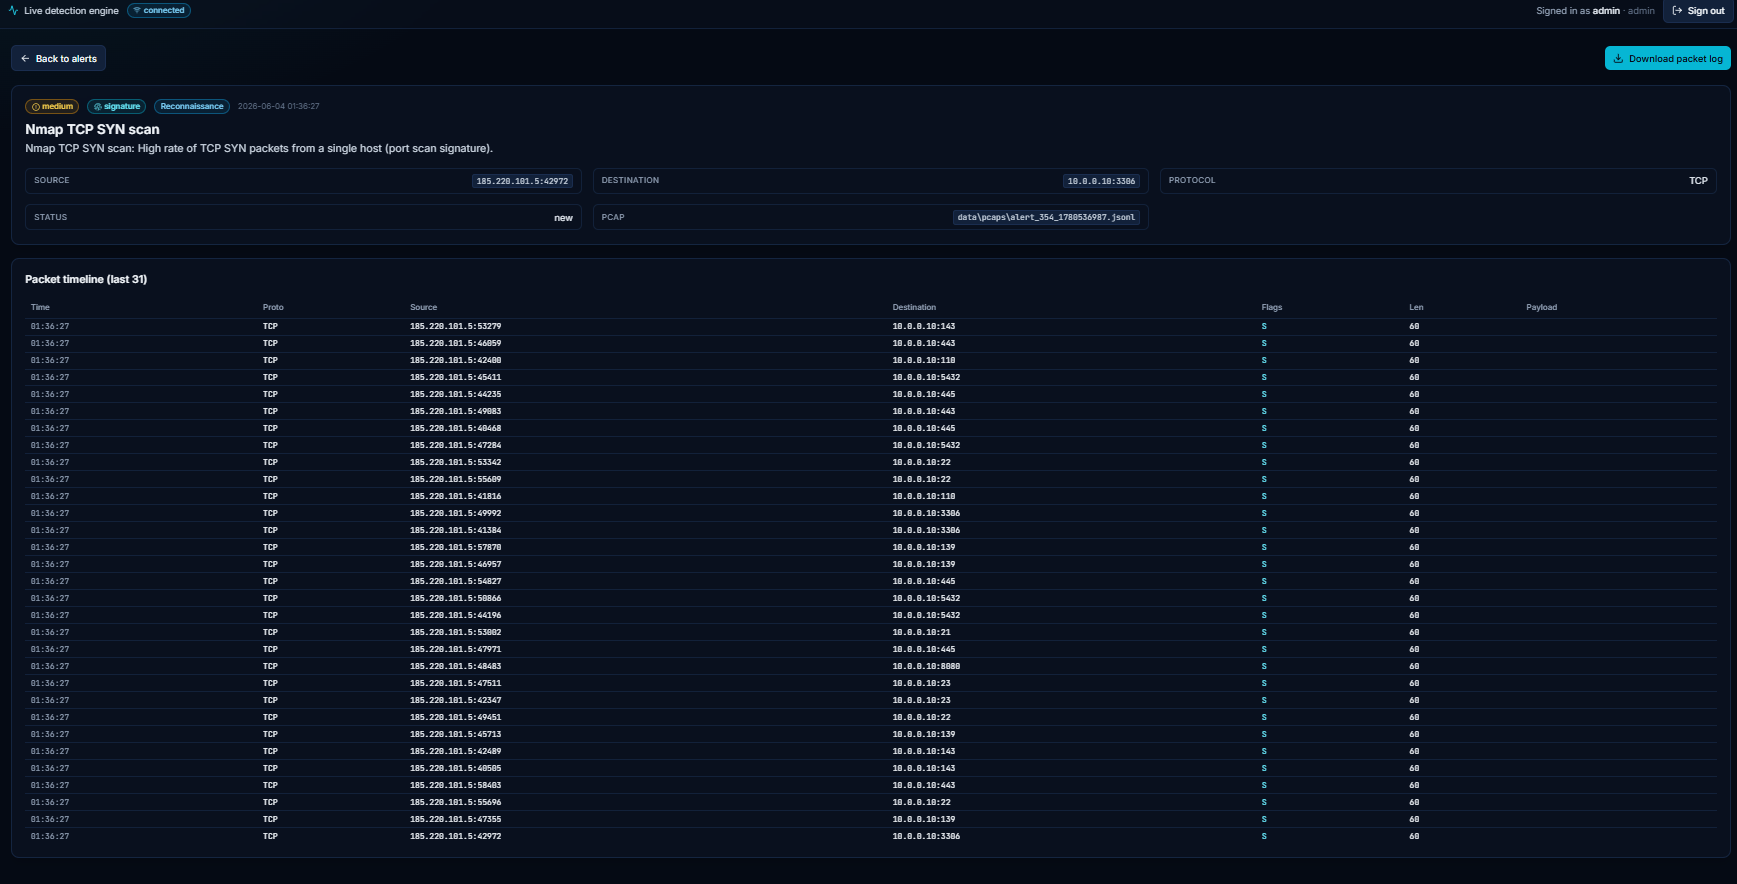
\includegraphics[width=\textwidth]{alert-detail}
\caption{The Alert Detail page for a single Nmap TCP SYN scan
alert. The header summarises the detection (severity, method,
category, timestamp); the metadata block lists the 5-tuple and
the path of the JSONL capture; and the packet timeline at the
bottom shows the last 31 packets captured around the alert, all
TCP SYN frames from the attacker hitting different destination
ports on the defended host --- the textbook signature of a port
scan.}
\label{fig:alert-detail}
\end{figure}

\textbf{Rules} (\file{Rules.jsx}) is the rule editor. Each rule
is a row in a table; clicking Edit opens the rule in a JSON
editor where the operator can adjust the match specification.
Saving triggers a hot reload of the in-memory rule list on the
backend. Deletion is gated by a themed confirmation dialog ---
a custom component matching the navy-and-cyan look of the rest
of the console, rather than the browser's native
\code{window.confirm} which broke the visual identity.

\begin{figure}[ht]
\centering
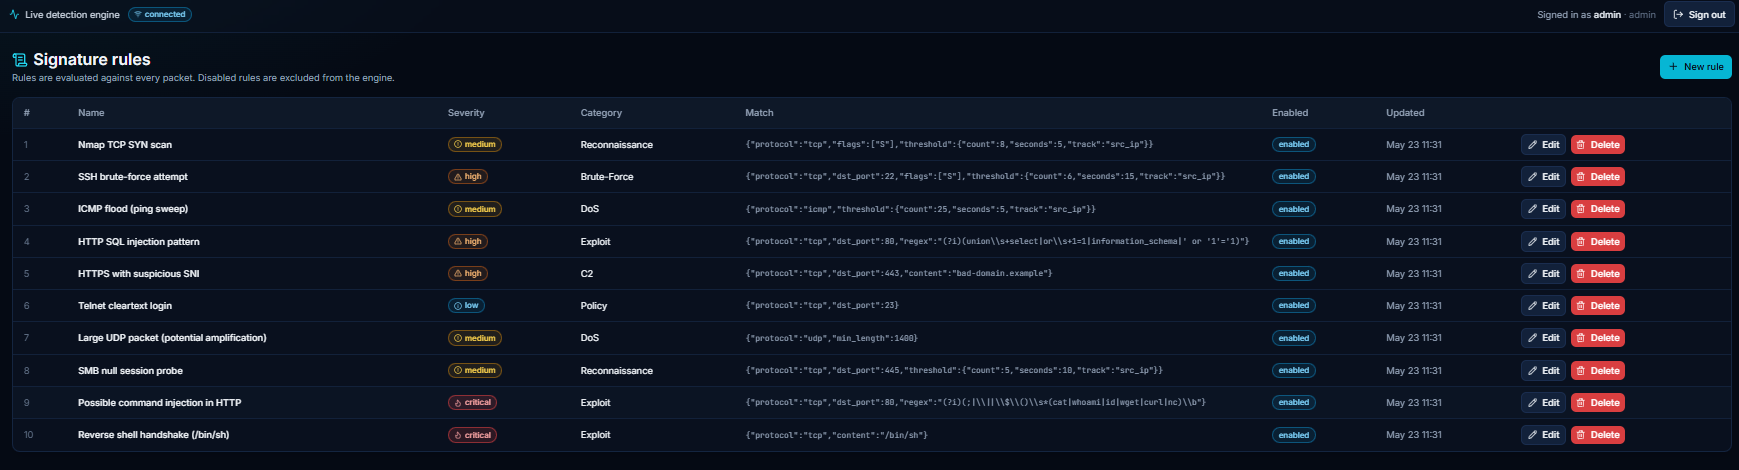
\includegraphics[width=\textwidth]{rules}
\caption{The Rules page listing the ten signature rules seeded
from \file{default\_rules.yaml}. The \code{Match} column shows
the raw JSON the engine evaluates; the Severity and Category
columns are visual cues for triage; Edit and Delete buttons on
each row mutate the database and reload the in-memory rule list
without a backend restart.}
\label{fig:rules}
\end{figure}

\textbf{ML Models} (\file{MLModels.jsx}) is the machine-learning
console. The left side has the training form (name and
algorithm dropdown), the right side shows the active model's
metrics and feature importance. A registry table at the bottom
lists all models with their accuracy and F1 scores. The page is
described in detail in Section~\ref{sec:design-ml} and
illustrated in Figure~\ref{fig:ml-models}.

\textbf{Attack Console} (\file{AttackConsole.jsx}) exposes the
six on-demand attacks as buttons, plus a toggle for the benign
traffic baseline. Each button click triggers
\code{POST /api/sim/attack} and shows the number of alerts
generated as a chip on the row. The Run All Attacks button
cycles through every attack with a half-second gap. The page is
described in detail in Section~\ref{sec:design-attack-console}
and illustrated in Figures~\ref{fig:attack-console}
and~\ref{fig:attack-console-fired}.

\textbf{Forensics} (\file{Forensics.jsx}) lists all PCAP
records in the database. Each row shows the file name, the
linked alert, the packet count and a Download button. See
Figure~\ref{fig:forensics} for the rendered view.

\textbf{Settings} (\file{Settings.jsx}) has three sections: an
Account section with a working change-password form, an Engine
Status panel refreshed every three seconds from
\code{/api/health}, and a Deployment Configuration reference
listing the environment variables and their effects.

\begin{figure}[ht]
\centering
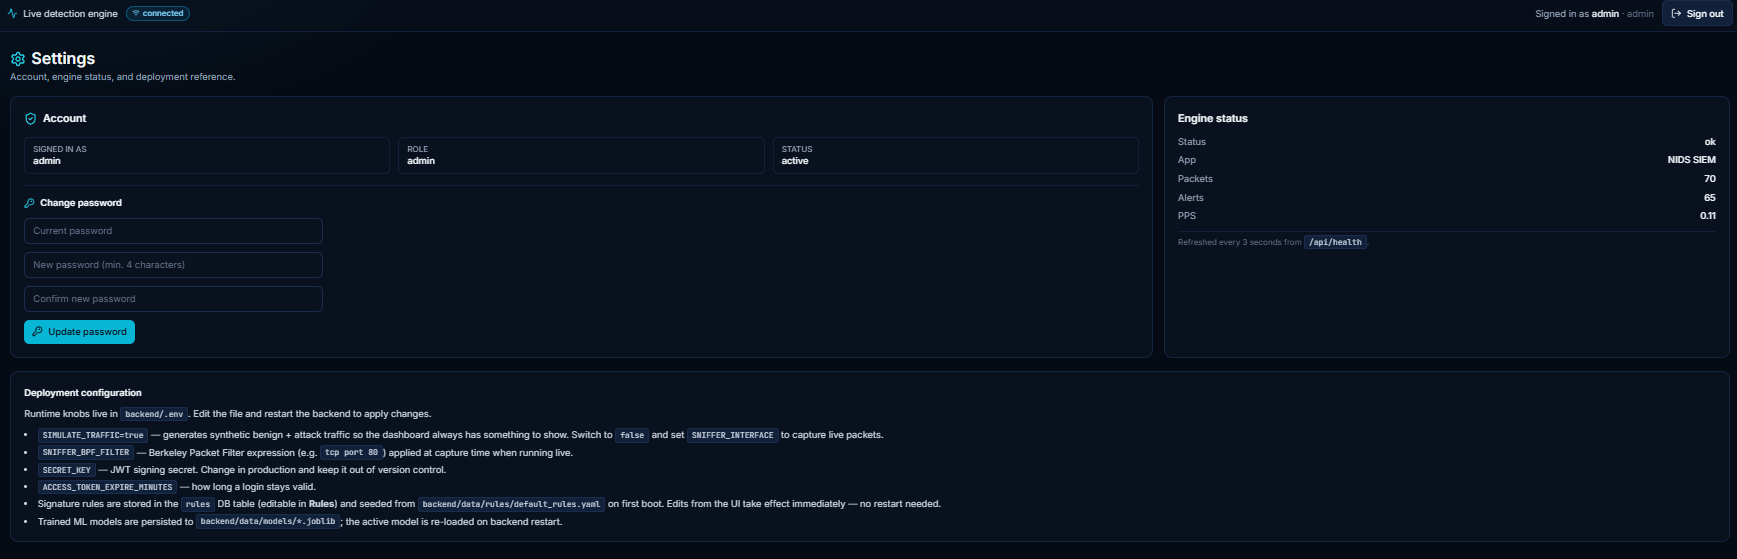
\includegraphics[width=\textwidth]{settings}
\caption{The Settings page. The Account panel on the left lets
the signed-in user rotate their own password (the form posts to
\code{POST /api/auth/change-password}, which re-verifies the
current password before writing a new bcrypt hash). The Engine
Status panel on the right polls \code{/api/health} every three
seconds; the Deployment Configuration block at the bottom is a
reference for which \file{.env} variables control which behaviour.}
\label{fig:settings}
\end{figure}

\section{Database Schema}
\label{sec:design-db}

The data model is small. The five tables are:

\begin{description}
  \item[users] (\file{models/user.py}) --- one row per account.
    Stores the bcrypt-hashed password, role, active flag and
    creation timestamp.
  \item[alerts] (\file{models/alert.py}) --- the central record.
    Carries severity, category, detection method, message,
    5-tuple, status, ML score, the path of the per-alert PCAP
    file, an extra JSON blob and the timestamp.
  \item[pcap\_records] (\file{models/pcap.py}) --- a denormalised
    view of the capture file for the Forensics page. Foreign
    keys the alert and stores the file name, full path,
    byte size and packet count.
  \item[traffic\_events] (\file{models/event.py}) --- sampled
    historical traffic. One row for every fifth packet seen.
  \item[rules] (\file{models/rule.py}) --- the rule database.
    \code{match} is a JSON column; everything else is small
    metadata.
  \item[ml\_models] (\file{models/ml\_model.py}) --- the
    registry of trained ML model artefacts. Name is unique;
    other columns are training metadata and the boolean
    \code{is\_active} flag.
\end{description}

Tables are created on first boot by
\code{Base.metadata.create\_all()} inside the FastAPI
\code{lifespan} handler. Schema migrations through Alembic are on
the future-work roadmap.

\section{Authentication Subsystem}
\label{sec:design-auth}

Authentication is a small but important subsystem. It comprises:

\begin{itemize}
  \item \file{backend/app/core/security.py}, which provides
    \code{hash\_password}, \code{verify\_password},
    \code{create\_access\_token} and \code{decode\_access\_token}.
  \item \file{backend/app/api/auth.py}, which exposes
    \code{POST /api/auth/login} (OAuth2 password flow),
    \code{GET /api/auth/me} (returns the signed-in user) and
    \code{POST /api/auth/change-password}.
  \item \file{backend/app/api/deps.py}, which holds
    \code{get\_current\_user} --- the FastAPI dependency every
    protected route uses.
\end{itemize}

The login flow is straightforward: the client posts a form-encoded
\code{username} and \code{password}, the endpoint looks up the
user, verifies the password against the stored bcrypt hash, and
issues a JWT signed with HS256. The token expires after one day
(configurable via \code{ACCESS\_TOKEN\_EXPIRE\_MINUTES}). The
frontend stores it in \code{sessionStorage} and attaches it to
every subsequent request as the
\code{Authorization: Bearer ...} header.

\section{The Attack Console (Red Team in a Box)}
\label{sec:design-attack-console}

The Attack Console deserves its own section because it is the
component that addresses the question ``does this system actually
demonstrate attacks?'' --- a question I was asked during the
project review.

The API surface is three endpoints in
\file{backend/app/api/sim.py}:
\code{GET /api/sim/info} returns the current state (defended
host, mode, attacks fired, available attack types);
\code{POST /api/sim/attack} fires one attack of a given kind;
\code{POST /api/sim/benign} toggles the benign baseline at
runtime.

The interesting behaviour is in the \code{POST /api/sim/attack}
handler. It captures the dispatcher's current alert count,
invokes \code{sim.fire\_attack(kind)} which routes the synthetic
packets through the dispatcher's
\code{handle()} exactly as if they had come from the network,
sleeps for 150\,ms to let the asynchronous database commits
settle, captures the new alert count and returns the delta in
the \code{alerts\_generated} field of the response. The frontend
displays the number as a chip on the recent-injections row, so
the operator sees instant confirmation that the attack actually
fired alerts. This was added specifically because during one of
the early demos I noticed that an attack could be fired but the
analyst had to switch tabs to verify alerts were generated; the
\code{alerts\_generated} field collapses that two-step
verification into one.

\begin{figure}[ht]
\centering
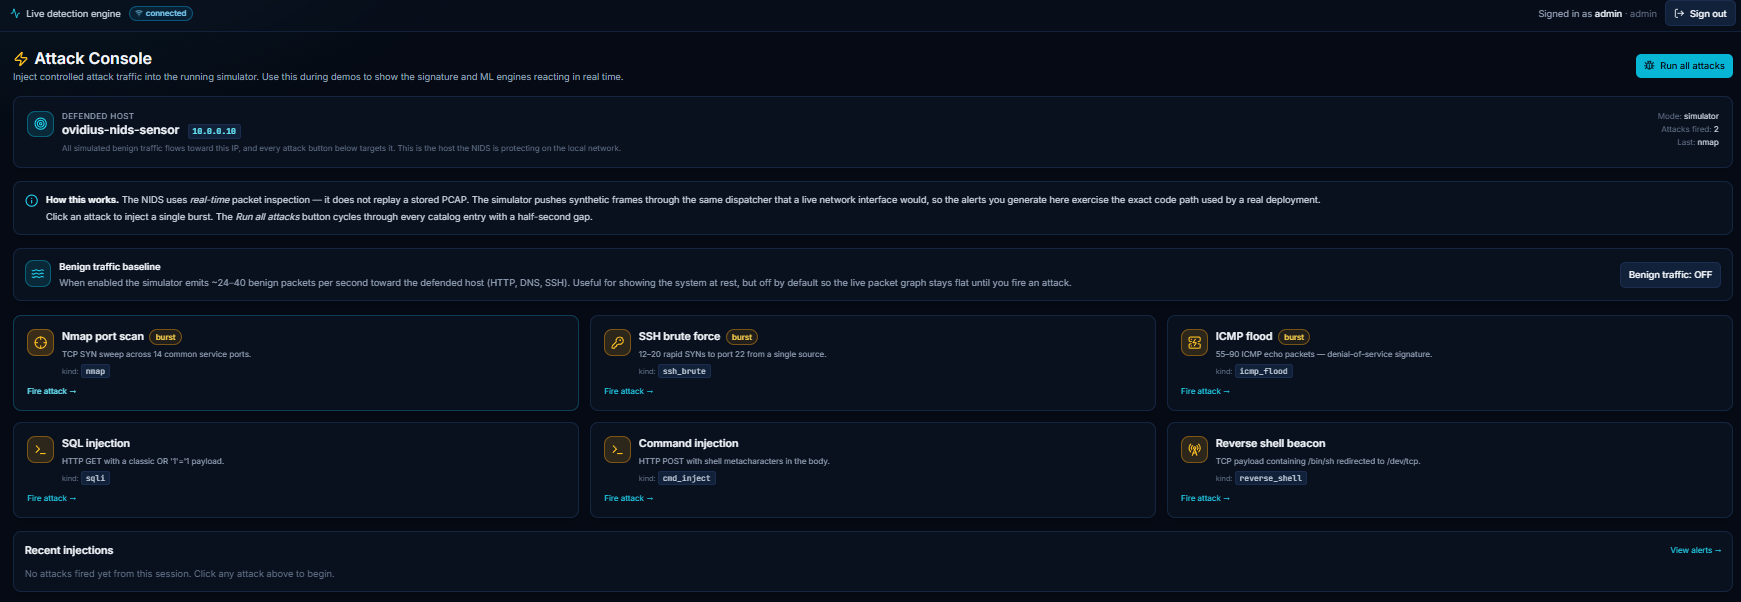
\includegraphics[width=\textwidth]{attack-console}
\caption{The Attack Console at rest. The Defended Host panel at
the top reports which IP every simulated attack will target; the
``How this works'' banner explains the real-time inspection
model; the Benign traffic baseline toggle is off by default so
the dispatcher sees no packets at all until an attack button is
clicked. The six attack cards expose the catalogue from
\code{TrafficSimulator.ATTACK\_CATALOG}.}
\label{fig:attack-console}
\end{figure}

\begin{figure}[ht]
\centering
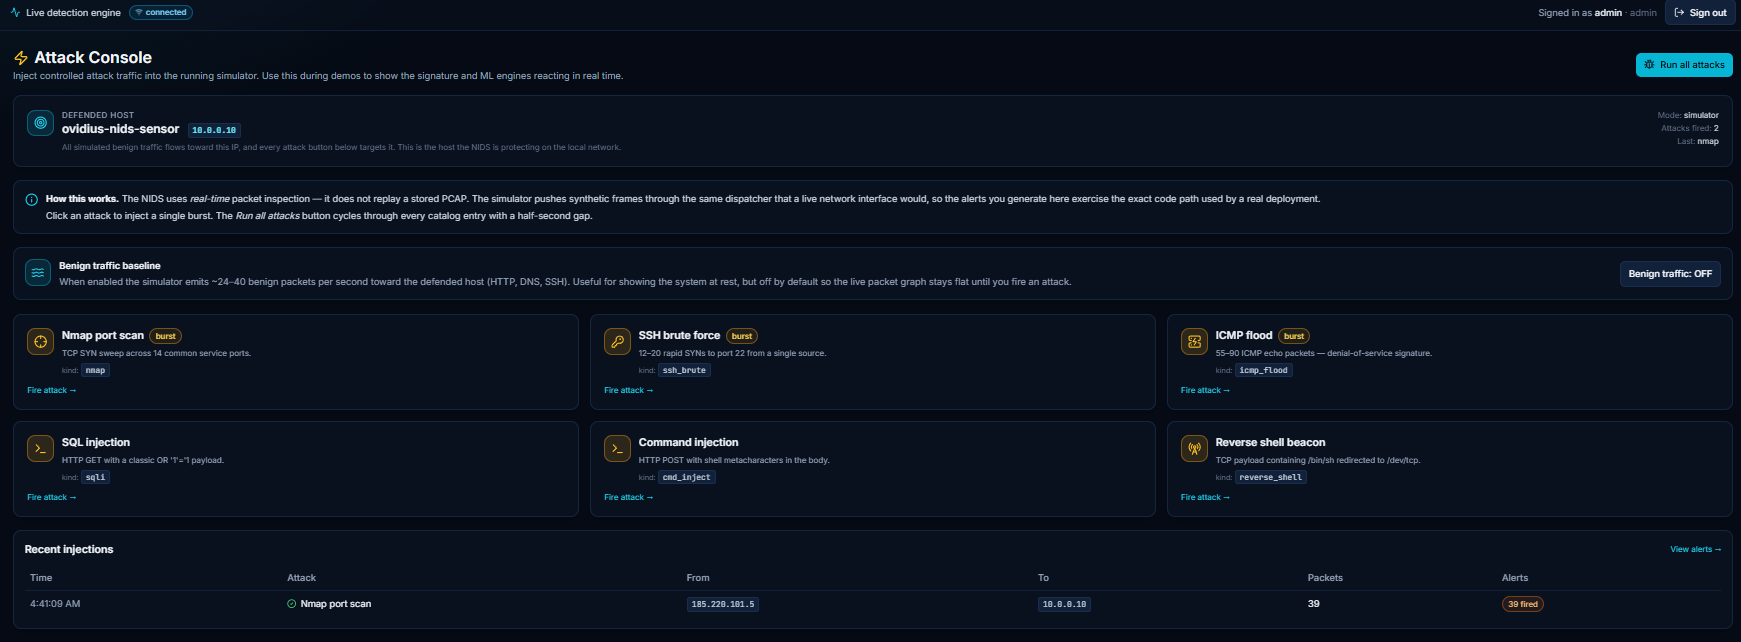
\includegraphics[width=\textwidth]{attack-console-after-fire}
\caption{The Attack Console immediately after the operator has
fired the Nmap port scan. The Recent Injections row at the bottom
shows the attacker IP from the simulator's pool
(\code{185.220.101.5}), the defended host as target
(\code{10.0.0.10}), 39 packets injected, and the green
\textit{39 fired} chip confirming the dispatcher produced 39
alerts from the burst. This per-attack feedback loop replaces
the older ``switch to the Alerts tab to check'' workflow.}
\label{fig:attack-console-fired}
\end{figure}

\section{The Cross-Platform Launcher}
\label{sec:design-launcher}

The launcher \file{run.py} (with the wrappers \file{run.bat} and
\file{run.sh}) is the front door of the project. It performs the
following operations, in order:

\begin{enumerate}
  \item Banner and Python-version check. Reject 3.14+.
  \item Ensure \file{backend/.env} exists, copy from
    \file{.env.example} if not.
  \item Create \file{backend/.venv/} if missing.
  \item Install Python dependencies from
    \file{requirements.txt} into the venv. Skip if the cached
    requirements hash matches.
  \item Verify the critical modules (uvicorn, fastapi,
    sqlalchemy, sklearn) actually import.
  \item Locate \code{npm} on PATH. If missing, fall back to
    backend-only mode.
  \item Install frontend dependencies via
    \code{npm install} if \file{node\_modules/} is missing.
  \item Start the FastAPI backend as a subprocess with
    \code{uvicorn app.main:app --host 0.0.0.0 --port 8000 --reload}.
  \item Start the Vite frontend as a subprocess with
    \code{npm run dev}.
  \item Wait for the frontend (or the backend Swagger UI in
    backend-only mode) to respond on its port.
  \item Open the URL in the default browser.
  \item Supervise the two subprocesses and stream their stdout
    into the launcher's terminal with colour-coded prefixes.
  \item On \code{SIGINT} (\verb|Ctrl+C|), invoke the idempotent
    \code{shutdown()} routine that politely signals both
    children and escalates to \code{kill} after a five-second
    grace period.
\end{enumerate}

The shutdown idempotency was a fix for an issue I noticed during
testing: \code{shutdown()} was being invoked three times in a
row (once by the signal handler, once by the \code{atexit}
registration, and once by the \code{finally:} clause in
\code{\_\_main\_\_}). On Windows, this caused the cmd.exe
``Terminate batch job? (Y/N)'' prompt to fire twice. The fix is a
one-line module-level flag that guards the body of
\code{shutdown()}.
